\documentclass[a4paper,12pt]{article}

\usepackage[utf8]{inputenc}
\usepackage{geometry}

\geometry{
    left=1cm,
    right=1cm,
    top=1.5cm,
    bottom=2.5cm
}

\usepackage{setspace}
\usepackage{xcolor}
\usepackage{tikz}
\usetikzlibrary{trees}

\definecolor{lightblue}{RGB}{124, 214, 235}
\definecolor{middleblue}{RGB}{38, 150, 201}
\definecolor{darkblue}{RGB}{49, 86, 148}

\begin{document}

\begin{center}
    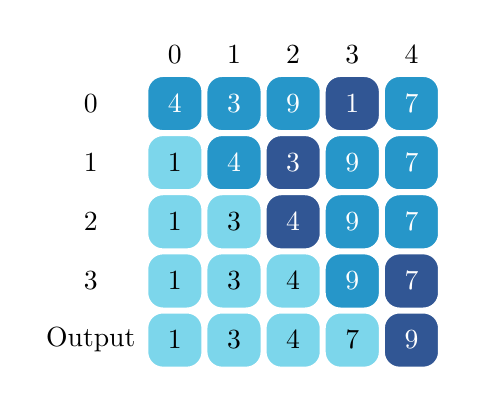
\begin{tikzpicture}[thick,
            light/.style = {draw=white, text=black, fill=lightblue,  rounded corners=2mm, minimum size=2em}, 
           middle/.style = {draw=white, text=white, fill=middleblue, rounded corners=2mm, minimum size=2em},
             dark/.style = {draw=white, text=white, fill=darkblue,   rounded corners=2mm, minimum size=2em}]
        \matrix [column sep=0.02cm, row sep=0.02cm]{
                	       & \node[] {$0$}; & \node[] {$1$}; & \node[] {$2$}; & \node[] {$3$}; & \node[] {$4$};\\
            \node[] {$0$}; & \node[middle] {$4$}; & \node[middle] {$3$}; & \node[middle] {$9$}; & \node[dark] {$1$}; & \node[middle] {$7$}; \\
            \node[] {$1$}; & \node[light] {$1$}; & \node[middle] {$4$}; & \node[dark] {$3$}; & \node[middle] {$9$}; & \node[middle] {$7$}; \\ 
            \node[] {$2$}; & \node[light] {$1$}; & \node[light] {$3$}; & \node[dark] {$4$}; & \node[middle] {$9$}; & \node[middle] {$7$}; \\ 
            \node[] {$3$}; & \node[light] {$1$}; & \node[light] {$3$}; & \node[light] {$4$}; & \node[middle] {$9$}; & \node[dark] {$7$}; \\ 
            \node[] {Output}; & \node[light] {$1$}; & \node[light] {$3$}; & \node[light] {$4$}; & \node[light] {$7$}; & \node[dark] {$9$}; \\ 
        };
    \end{tikzpicture}

    \footnotesize Example: SelectionSort
\end{center}

\end{document}